%!TEX root = ../dissertation.tex
\begin{savequote}[75mm]
There are some things you learn best in calm, and some in storm.
\qauthor{Willa Cather}
\end{savequote}

\chapter{Apache Storm}

Apache Storm is a reliable, distributed and fault-tolerant system for stream processing.
The beginnings of the project were at Backtype (later bought by Twitter) and created by Nathan Marz.
He open sourced Storm on September the 19th in 2011. The project rapidly got a big development coummunity and
on September the 18, 2013 Nathan moved Storme to Apache Incubator.\\

Storm works with different types of components which are responsible for clear defined task.
The components are bundled and managed in a so called \textbf{Topology}.
The entrypoint and the stream input is handled by a \textbf{Spout}, the spout passes data to the \textbf{Bolts}.
Bolts are responsible for the main data processing and persists the data.
They can be chained or parallelised in a way that fits best for your current problem.

\begin{figure}[H]
\centering
\captionsetup{justification=centering}
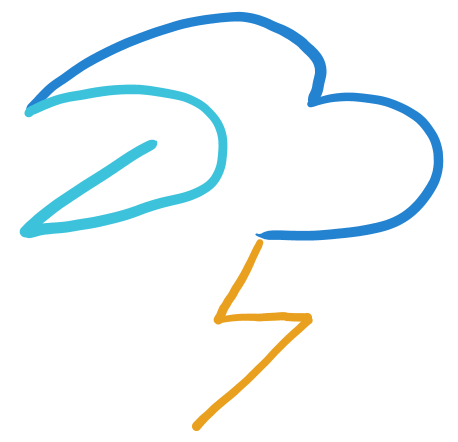
\includegraphics[width=80pt]{images/storm.png}
\caption[Storm]{Storm}
\end{figure}

\newpage

\section{Topology}
In generell Storm passes tuples between the different components.
To organize the tuples there are topologies.
\begin{figure}[H]
\centering
\captionsetup{justification=centering}
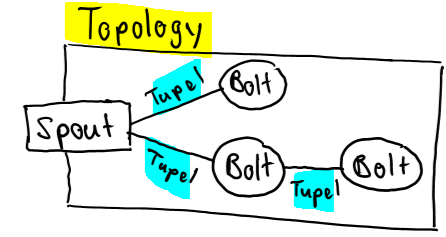
\includegraphics[width=0.4\textwidth]{images/topology_example.png}
\caption[Topology example]{Topology example}
\end{figure}

\subsection{Grouping}
The Topology defines the grouping, this means how streams are consumed by the bolts and how they consume them.
There are four kinds of grouping \textit{Shuffle Grouping}, \textit{Fields Grouping},
\textit{All Grouping} and \textit{Custom Grouping}.

\subsubsection{Shuffle Grouping}
Shuffle Grouping takes a single entry from the source and sends each tuple to a randomly choosen bolt,
which is listening to this kind of tuples. It also garanties that each consumer gets more or less the same number of tuples.

\subsubsection{Fields Grouping}
With Fields Grouping it is possible to send tuples to spezified bolts based on the fields of the tuple.
It takes care that the same combination of fields is always sent to the same bolt.

\subsubsection{All Grouping}
All Grouping sends every tuple to all the bolts. This is helpful for tasks like signals or to
use different filters for alerting systems working on the same input.

\subsubsection{Custom Grouping}
It is possible to build your on grouping based on the stream. This is very helpful if you have to make
fine granular desicions about which bolt has to handle which tuple.


\newpage

\section{Spout}
The entry point of each topology are the so called spouts. Their main task is to procure the data from the input source.
After the access of the source the spout emits a list of defined fields, which are consumed by the bolts.
The spouts are also responsible for reliability,
thus you have to take care to implement them in a fault-tolerant way. This means that a spout must have the
ability to deal with unprocessable and unpredictable messages from the stream.\\
To handle the reliability at the spout you can add an ID to every message. If a message is correctly processed  by
all the target bolts the \textit{ack} method of the spout is called. But if there were troubles or the timeout is
reached the \textit{fail} method will be triggered.

\subsubsection{Example}
As an example you can imagine a spout which consumes data from a message queue and emits the data
to the interessted bolts. All of this data steam is defined in the Storm topology.

\begin{figure}[H]
\centering
\captionsetup{justification=centering}
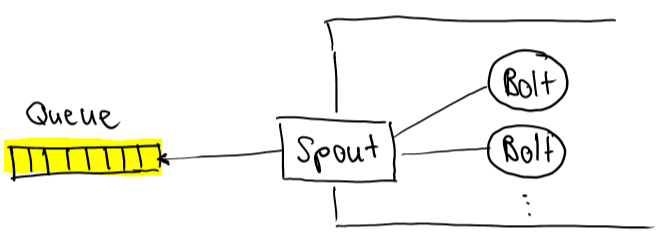
\includegraphics[width=0.4\textwidth]{images/spout_example.png}
\caption[Spout example]{Spout example}
\end{figure}

\subsubsection{Code}
And in the code this could look like the following.
\begin{lstlisting}
TopologyBuilder builder = new TopologyBuilder();
MessageQueueSpout spout = new MessageQueueSpout();
PrinterBolt bolt = new PrinterBolt();

builder.setSpout("spout", spout);
builder.setBolt("bolt", bolt).shuffleGrouping("spout");
\end{lstlisting}


\newpage

\section{Bolt}
Bolts are the heartpieces, the engine of Apache Storm, they are responsible for the hard work of processing the data.
A bolt takes tuples as input, does some operations on it and finally produces tuples as output.
Normally a bolt implements the \textit{IRichBolt} interface, which has the following methods.

\begin{figure}[H]
\centering
\captionsetup{justification=centering}
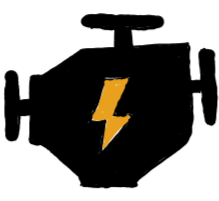
\includegraphics[width=0.2\textwidth]{images/engine.png}
\caption[Bolt engine]{Bolt engine}
\end{figure}

\subsubsection{Methods}
A Bolt provides the following basic methods.
\begin{enumerate}
    \item void prepare(Map map, TopologyContext topologyContext)
    \item void execute(Tuple tuple, BasicOutputCollector basicOutputCollector)
    \item void declareOutputFields(OutputFieldsDeclarer outputFieldsDeclarer)
    \item void cleanup()
\end{enumerate}

\subsubsection{prepare}
This method is always called befor the bolts starts to process tuples\\ (before the execute method)).
A possible task could be to reset a counter.


\subsubsection{execute}
The execute methode processes a singel tuple of input, so it is the core function of every bold.
So all the logic should be done here, for example filter a stream or counting the words of the input.

\subsubsection{declareOutputFields}
The prepare method is responsible for defining the output schema of the bolt.
If bolts are concatenated the output is a tuple ,but if the current bolt is may be the last bolt in the chain,
and does a task like, print to the standard output, you don't have to set an output type.

\subsubsection{cleanup}
Cleanup() is called when a bolt is going to shutdown. So you should do some tasks like a destructor does.
For example disconnect an active database connection.
